\chapter{Sistema de abastecimento}

\section{Lista de materiais}
\begin{table}[H]
\centering
\begin{tabular}{|m{2.0cm} |m{9.2cm}|m{2.0cm}|}
\hline
\begin{center}Quantidade\end{center} & \begin{center}Componente\end{center} &\begin{center} Identificador\end{center} \\\hline

    02 & Chapa de aço carbono SAE 1020 de 500mm x 400mm x 2mm & 01 \\\hline
    04 & Porca sextavada M8x15cm & 02 \\\hline
    01 & Tarugo de aço SAE 1045 de 15 mm de diâmetro & 03 \\\hline
    
    
\end{tabular}
\label{table: tabelaComponentesMaletaControle}
\caption{Lista de componentes}
\end{table}

\section{Ferramentas}
    \par Para a montagem da capa protetora da estrutura do sistema válvula-atuador:
    \begin{itemize}
        \item Serra circular para metais
        \item Dobradeira de chapa
        \item Maquina inversora de solda
        \item Furadeira
        \item Broca aço rápido de 5 mm
        \item Broca aço rápido de 10 mm
        \item Serra copo de 20 mm para metais
    \end{itemize}
    
        \par Para a montagem do pino de acoplamento do motor à válvula:
    \begin{itemize}
        \item Serra circular para metais
        \item Torno automático de eletroerosão
        \item Furadeira de bancada 
        \item Broca aço rápido de 5 mm
    \end{itemize}

\section{Fabricação da capa protetora da estrutura do sistema válvula-atuador}
A capa protetora da estrutura é composta por duas partes inteiriças: uma chapa de aço forma a parte superior onde é fixado o motor, e a outra chapa forma a parte inferior onde devem ser fixado os mancais.

Para a fabricação da parte superior da capa, utilizar serra circular para aço para cortar a chapa e obter o resultado de acordo com a figura a seguir:
\begin{figure} [H]
    \centering
    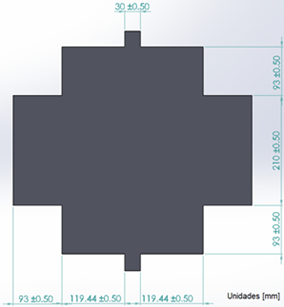
\includegraphics[width=.5\textwidth]{Figuras/montagemAbastecimento/capa/etapa1.png}
    \caption{Etapa 1 da fabricação da capa protetora da estrutura do sistema válvula-atuador - Vista superior}
    \label{fig:etapa1}
\end{figure}

A seguir, realizar conformação mecânica por meio de dobras utilizando a dobradeira ou outra ferramenta adequada e unir as arestas soltas por meio de soldagem convencional para se obter o seguinte resultado:
\begin{figure} [H]
    \centering
    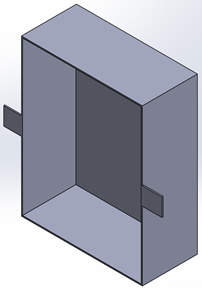
\includegraphics[width=.3\textwidth]{Figuras/montagemAbastecimento/capa/etapa2.png}
    \caption{Etapa 2 da fabricação da capa protetora da estrutura do sistema válvula-atuador - Visão isométrica da vista inferior}
    \label{fig:etapa2}
\end{figure}

 Em seguida, utilizar a furadeira para fazer dois furos de 10 mm de diâmetro, sendo um furo em cada uma das aletas de fixação. O furo deve estar no centro da aleta de fixação. Em seguida, realizar abaulamento das quinas com a serra circular, resultando em uma estrutura semelhante a figura abaixo:
\begin{figure} [H]
    \centering
    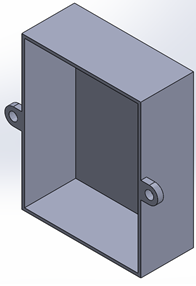
\includegraphics[width=.3\textwidth]{Figuras/montagemAbastecimento/capa/etapa3.png}
    \caption{Etapa 3 da fabricação da capa protetora da estrutura do sistema válvula-atuador - Visão isométrica da vista inferior}
    \label{fig:etapa3}
\end{figure}

Com uma serra-copo de 20 mm de diâmetro, realizar o furo da passagem dos cabos de acionamento do motor. A face a ser furada é a face da esquerda, de acordo com a imagem:
\begin{figure} [H]
    \centering
    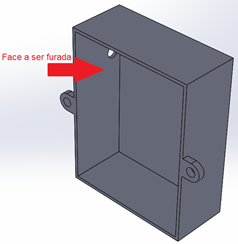
\includegraphics[width=.4\textwidth]{Figuras/montagemAbastecimento/capa/etapa4_1.png}
    \caption{Etapa 4.1 da fabricação da capa protetora da estrutura do sistema válvula-atuador - Visão isométrica da vista inferior}
    \label{fig:etapa4.1}
\end{figure}

A posição do furo na face deve ser atentamente marcada de acordo com o observado na figura abaixo:
\begin{figure} [H]
    \centering
    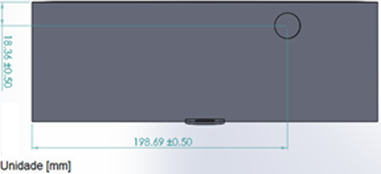
\includegraphics[width=.5\textwidth]{Figuras/montagemAbastecimento/capa/etapa4_2.png}
    \caption{Etapa 4.2 da fabricação da capa protetora da estrutura do sistema válvula-atuador - Vista lateral esquerda}
    \label{fig:etapa4.1}
\end{figure}

Com a serra circular, realizar dois cortes no formato de meia circunferência que servem de para a passagem da tubulação. A figura a seguir mostra os locais dos cortes:
\begin{figure} [H]
    \centering
    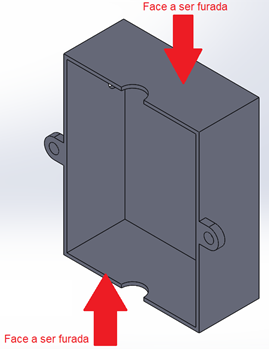
\includegraphics[width=.4\textwidth]{Figuras/montagemAbastecimento/capa/etapa5_1.png}
    \caption{Etapa 5.1 da fabricação da capa protetora da estrutura do sistema válvula-atuador - Visão isométrica da vista inferior}
    \label{fig:etapa5.1}
\end{figure}

A posição do corte na face deve ser atentamente marcada de acordo com o observado e os furos em cada face devem estar alinhados. A figura a seguir mostra a posição de cada corte:
\begin{figure} [H]
    \centering
    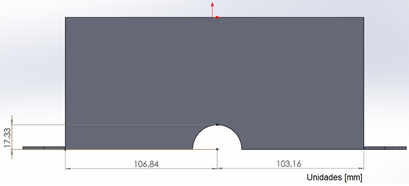
\includegraphics[width=.7\textwidth]{Figuras/montagemAbastecimento/capa/etapa5_2.png}
    \caption{Etapa 5.2 da fabricação da capa protetora da estrutura do sistema válvula-atuador - Vista frontal}
    \label{fig:etapa5.2}
\end{figure}

Com o auxílio de uma furadeira equipada com broca de 5 mm, fazer quatro furos que serviram de suporte para o motor. Os furos estão localizados na face indicada:

\begin{figure} [H]
    \centering
    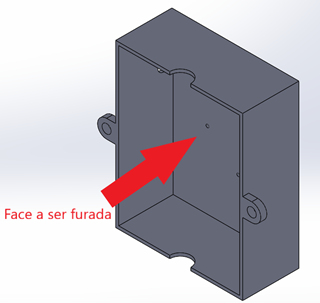
\includegraphics[width=.5\textwidth]{Figuras/montagemAbastecimento/capa/etapa6_1.png}
    \caption{Etapa 6.1 da fabricação da capa protetora da estrutura do sistema válvula-atuador - Visão isométrica da vista inferior}
    \label{fig:etapa6.1}
\end{figure}

A posição dos furos devem ser atentamente marcada e tomar como referência o furo de passagem dos cabos de acionamento do motor, conforme mostrado na figura seguir. É recomendada a checagem da marcação antes da execução dos furos.
\begin{figure} [H]
    \centering
    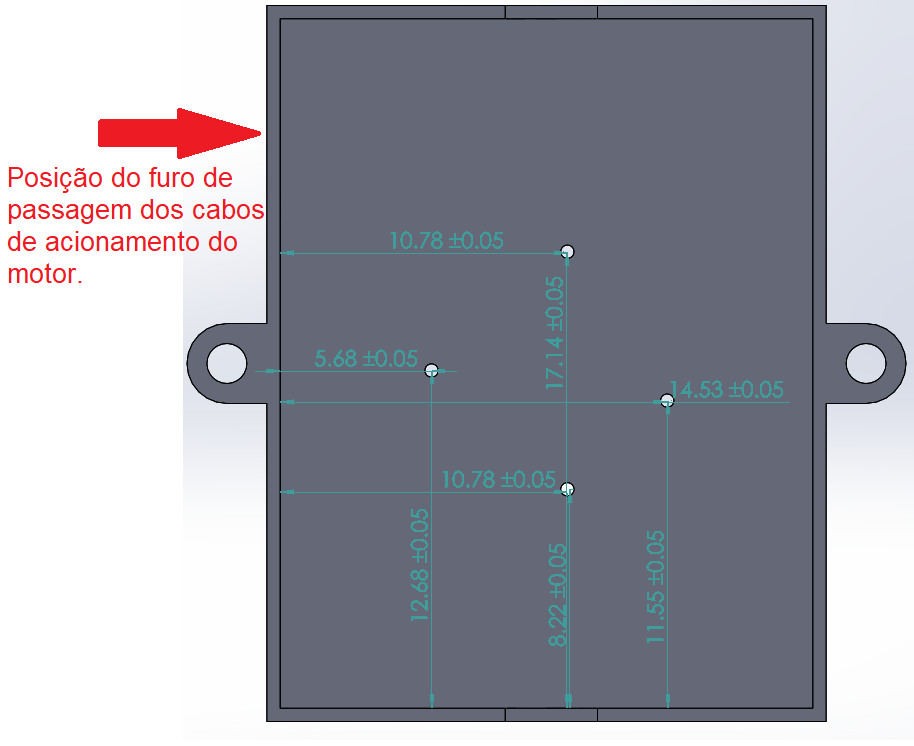
\includegraphics[width=.6\textwidth]{Figuras/montagemAbastecimento/capa/etapa6_2.png}
    \caption{Etapa 6.2 da fabricação da capa protetora da estrutura do sistema válvula-atuador - Visão inferior}
    \label{fig:etapa6.2}
\end{figure}

A parte superior é finalizada. Prosseguir para a fabricação da parte inferior da capa, utilizar uma serra circular para aço e cortar a chapa para que fique de acordo com a figura a seguir:
\begin{figure} [H]
    \centering
    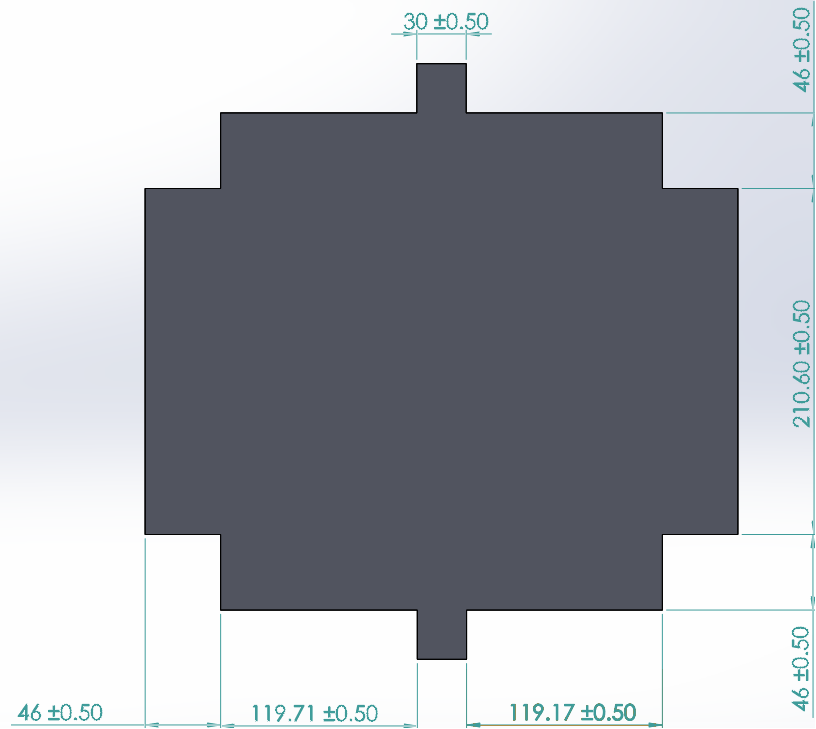
\includegraphics[width=.6\textwidth]{Figuras/montagemAbastecimento/capa/etapa7.png}
    \caption{Etapa 7 da fabricação da capa protetora da estrutura do sistema válvula-atuador - Vista superior}
    \label{fig:etapa7}
\end{figure}

Realizar os procedimentos de maneira semelhante a parte superior da capa de proteção. Conformação mecânica por meio de dobras utilizando a dobradeira ou outro material adequado e unir as arestas soltas por meio de soldagem convencional e utilizar a furadeira para fazer dois furos de 10 mm de diâmetro, sendo um furo em cada uma das aletas de fixação. O furo deve estar no centro da aleta de fixação. Em seguida, realizar abaulamento das quinas com a serra circular, resultando em uma estrutura semelhante a figura abaixo:
\begin{figure} [H]
    \centering
    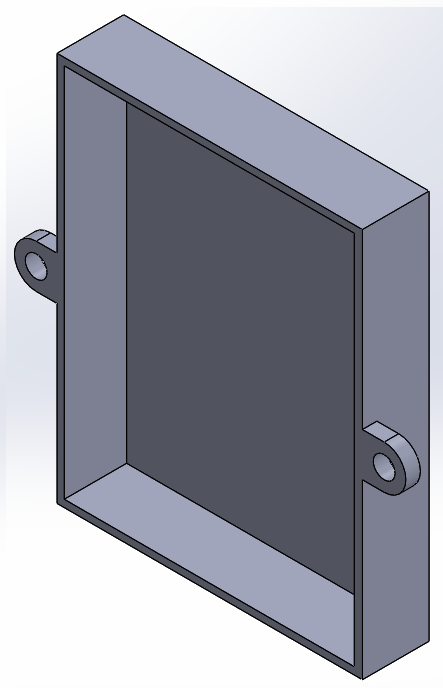
\includegraphics[width=.25\textwidth]{Figuras/montagemAbastecimento/capa/etapa8.png}
    \caption{Etapa 8 da fabricação da capa protetora da estrutura do sistema válvula-atuador - Visão isométrica da vista superior}
    \label{fig:etapa8}
\end{figure}

Com a serra circular, realizar dois cortes no formato de meia circunferência que servem de passagem para a tubulação. A posição do corte na face deve ser atentamente marcada tendo como referência a parte superior da capa. Posicione ambas partes encaixadas e marque a região do corte de maneira a formar uma circunferência completa com o arco de circunferência já existente. A figura a seguir mostra o resultado:
\begin{figure} [H]
    \centering
    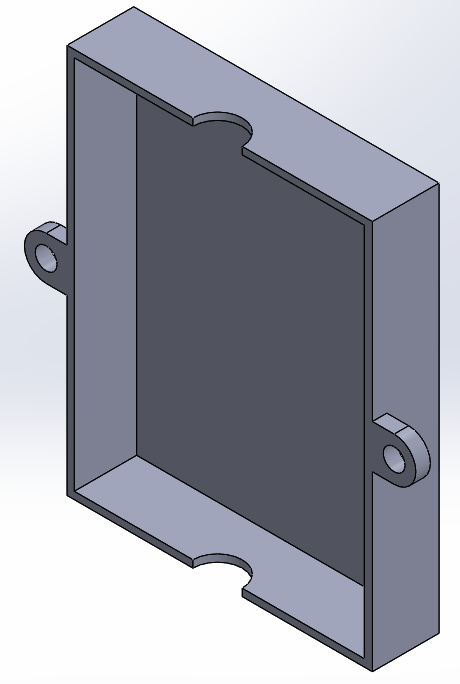
\includegraphics[width=.25\textwidth]{Figuras/montagemAbastecimento/capa/etapa9.png}
    \caption{Etapa 9 da fabricação da capa protetora da estrutura do sistema válvula-atuador - Visão isométrica da vista superior}
    \label{fig:etapa9}
\end{figure}

Para a fixação dos pontos de apoio dos mancais, realizar a união de quatro porcas sextavada M8x15cm com a parte inferior por meio de soldagem convencional. A superfície da porca deve estar paralela a superfície da chapa de aço. A posição dos furos devem ser atentamente marcada e tomar como referência o furo de passagem dos cabos de acionamento do motor (realizar o acoplamento das partes) conforme mostrado na figura seguir. É recomendada a checagem da marcação antes da execução dos furos.

\begin{figure} [H]
    \centering
    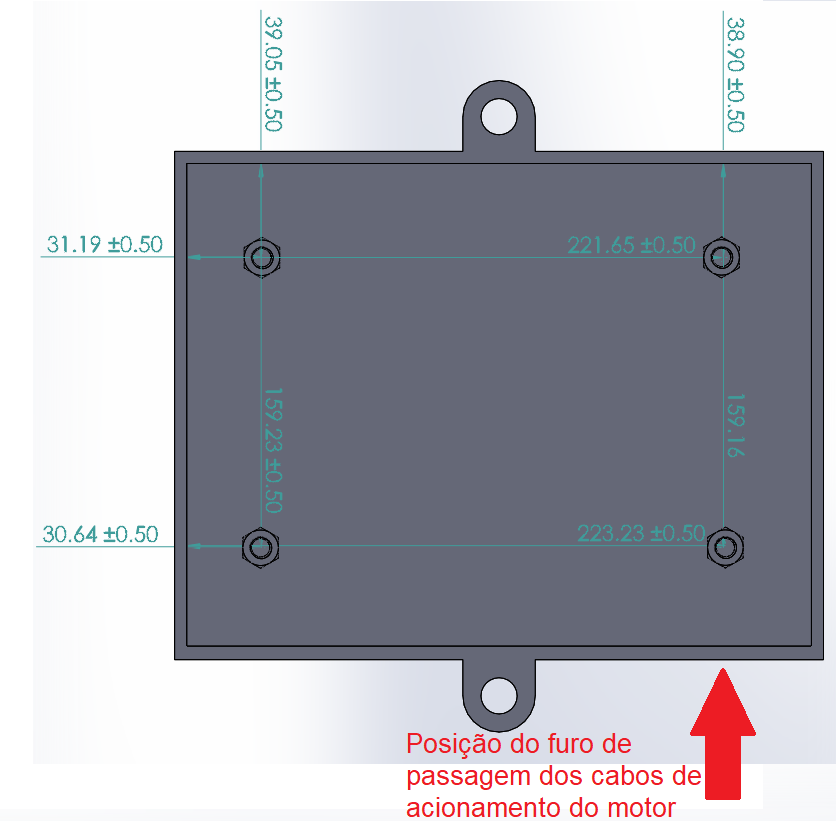
\includegraphics[width=.6\textwidth]{Figuras/montagemAbastecimento/capa/etapa10.png}
    \caption{Etapa 10 da fabricação da capa protetora da estrutura do sistema válvula-atuador - Vista superior}
    \label{fig:etapa10}
\end{figure}
 
\section{Fabricação do pino de acoplamento do motor à válvula}
Um tarugo de aço SAE 1045 de 15 mm de diâmetro é utilizado como matéria prima para a fabricação do pino. Cortar o tarugo para obter um segmento de 31.9 mm de comprimento, conforme a figura a seguir. 

\begin{figure} [H]
    \centering
    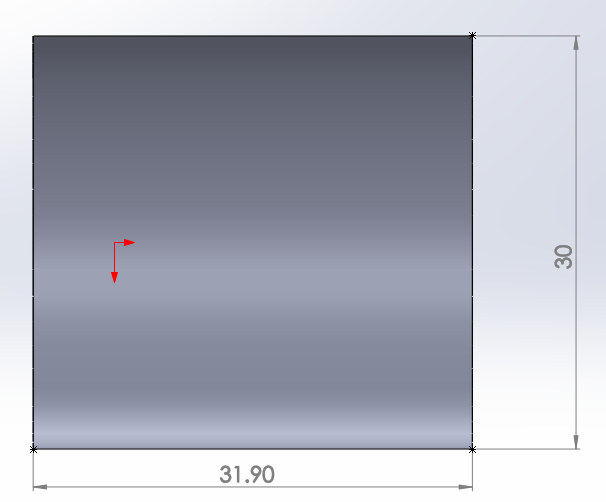
\includegraphics[width=.4\textwidth]{Figuras/montagemAbastecimento/pino/etapa1.png}
    \caption{Etapa 1 da fabricação do pino de acoplamento do motor à válvula - Vista lateral}
    \label{fig:pinoetapa1}
\end{figure}

Realizar os furos de acoplamento através do método de usinagem por eletroerosão. A retirada de material do tarugo deve ocorrer em três partes. A primeira parte feita em uma das faces planas do tarugo possui formato hexagonal regular assemelhado ao da porca que movimenta o comando da válvula esfera. 

\section{Montagem sistema válvula-atuador}

\begin{figure} [H]
    \centering
    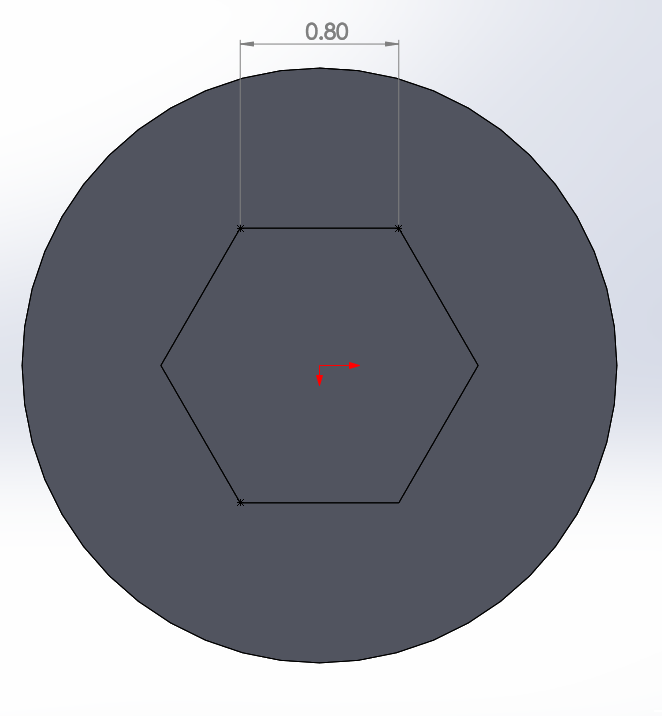
\includegraphics[width=.4\textwidth]{Figuras/montagemAbastecimento/pino/etapa2.png}
    \caption{Etapa 2 da fabricação do pino de acoplamento do motor à válvula - Vista inferior}
    \label{fig:pinoetapa2}
\end{figure}

A segunda parte é feita na face oposta e que deve levar o formato da engrenagem do motor elétrico. 

A terceira região a ser usinada consiste em um furo circular de  com rosca localizado na lateral do pino correspondente ao encaixe da válvula, de maneira que forme espaço utilizado pela trava guia do pino. A figura a seguir mostra o resultado

\begin{figure} [H]
    \centering
    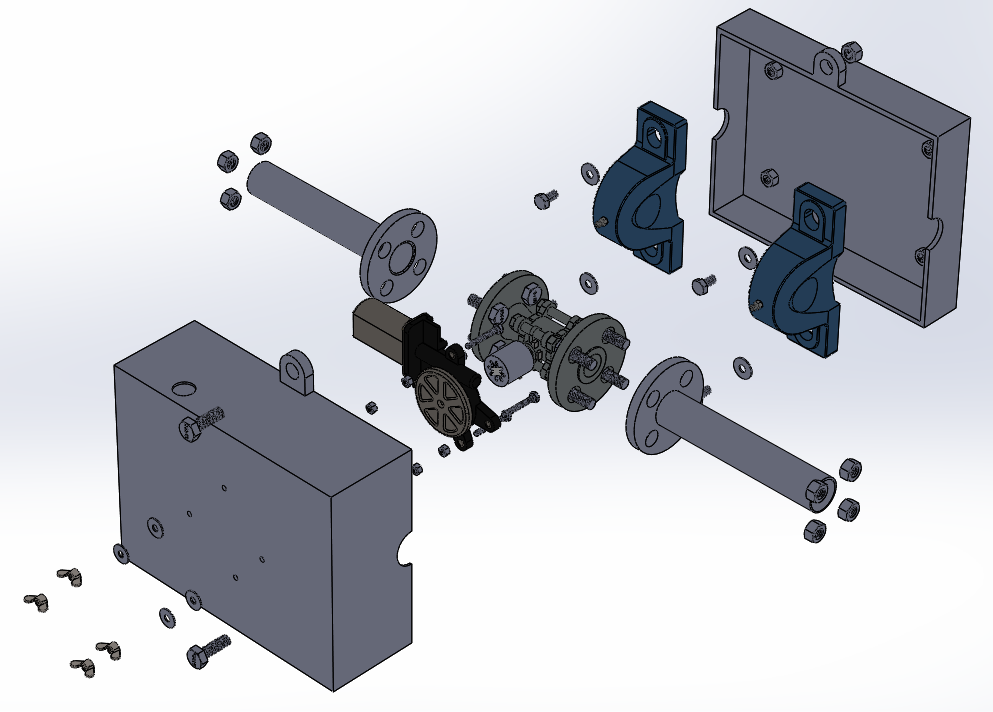
\includegraphics[width=1\textwidth]{Figuras/explodida_valvula.png}
    \caption{Vista explodida do adaptador}
\end{figure}

\begin{figure} [H]
    \centering
    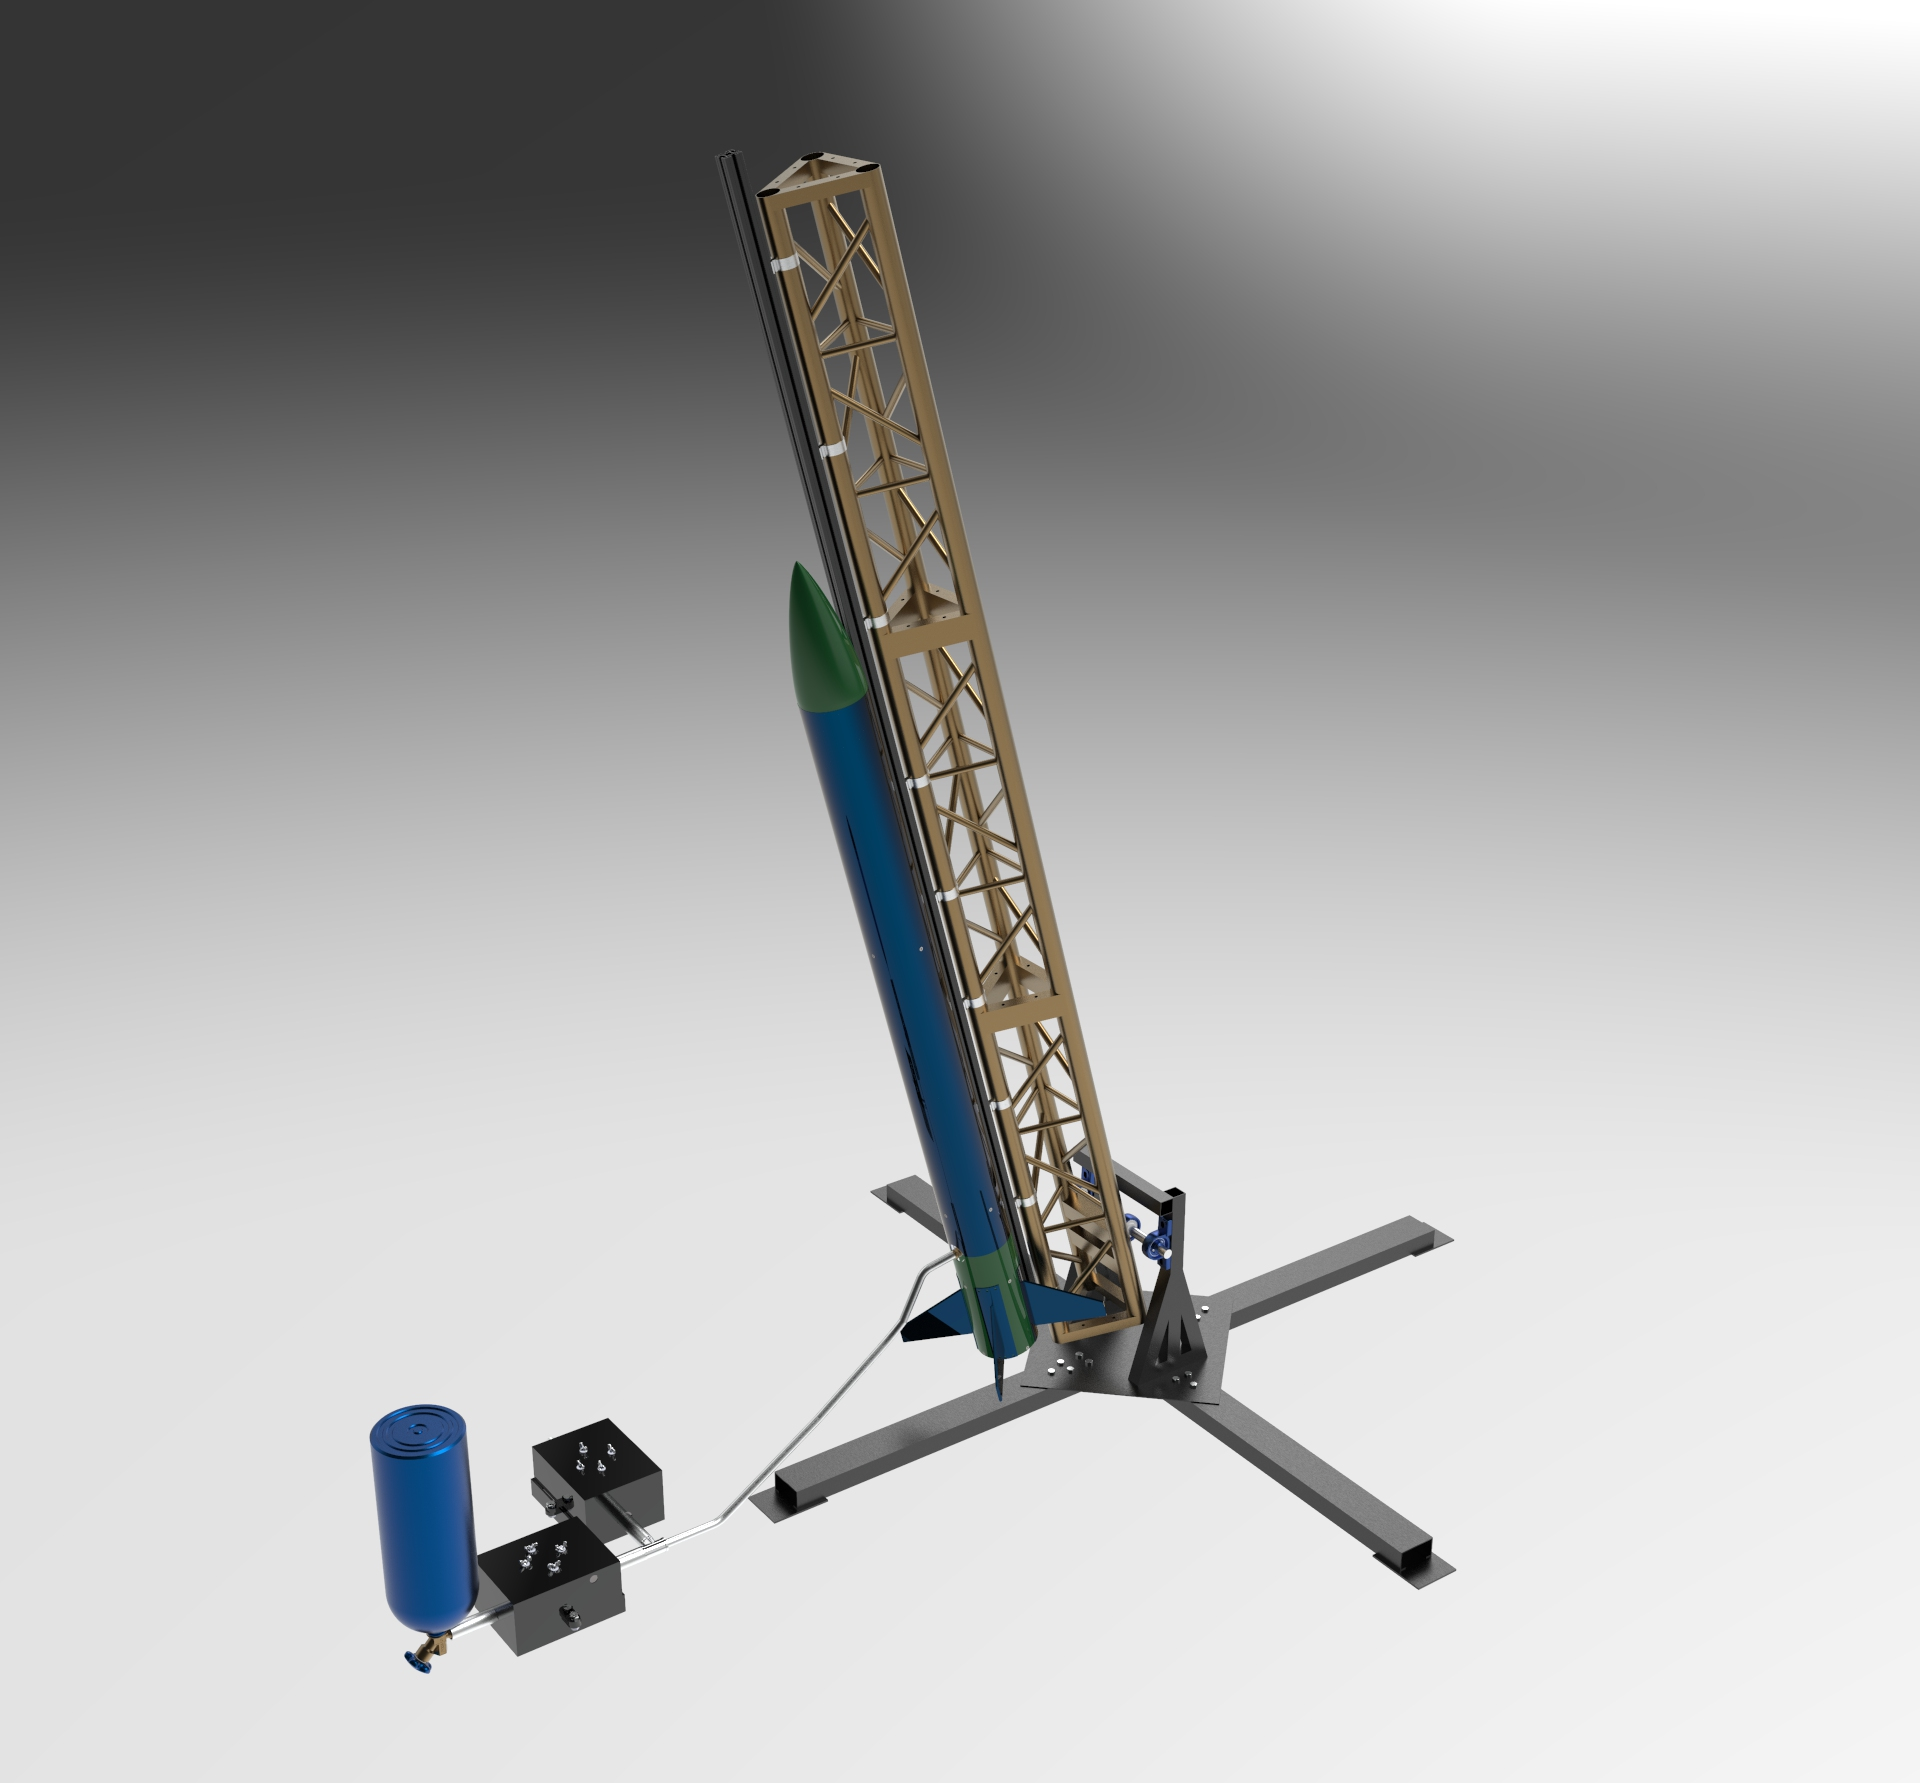
\includegraphics[width=1\textwidth]{Figuras/rend_alimentacao.31.jpg}
    \caption{Montagem completa do abastecimento}
\end{figure}
